\chapter{Results}
\label{resultschap}

In this section we present the results of the implementation of all the elements presented in chapter \ref{ch:tec}.

\section{Perception}

The culmination of the proximity sensor transformation explained in section \ref{s:perception}, in addition to the work done in calibration by the calibration group in the HIRO Lab, led by Kandai Watanabe, will allow to the robot to sense its surroundings.

In simulation, we show below that proximity sensors placed in the robot body (marked in red in figure \ref{fig:sensorssimulation}) can detect objects in simulation. In figure \ref{fig:visualizationpoints}, \lstinline{rviz} is placed on the left and the simulation in \lstinline{Gazebo} on the right. A black box is moved around in \lstinline{Gazebo} and the robot's perception, result of the transformation algorithm proposed in this work, is seen in \lstinline{rviz}.


\begin{figure}[H]
    \caption[Spheres]{
    Final visualization of the perceived points in \textit{rviz}.
    }
    \begin{center}
    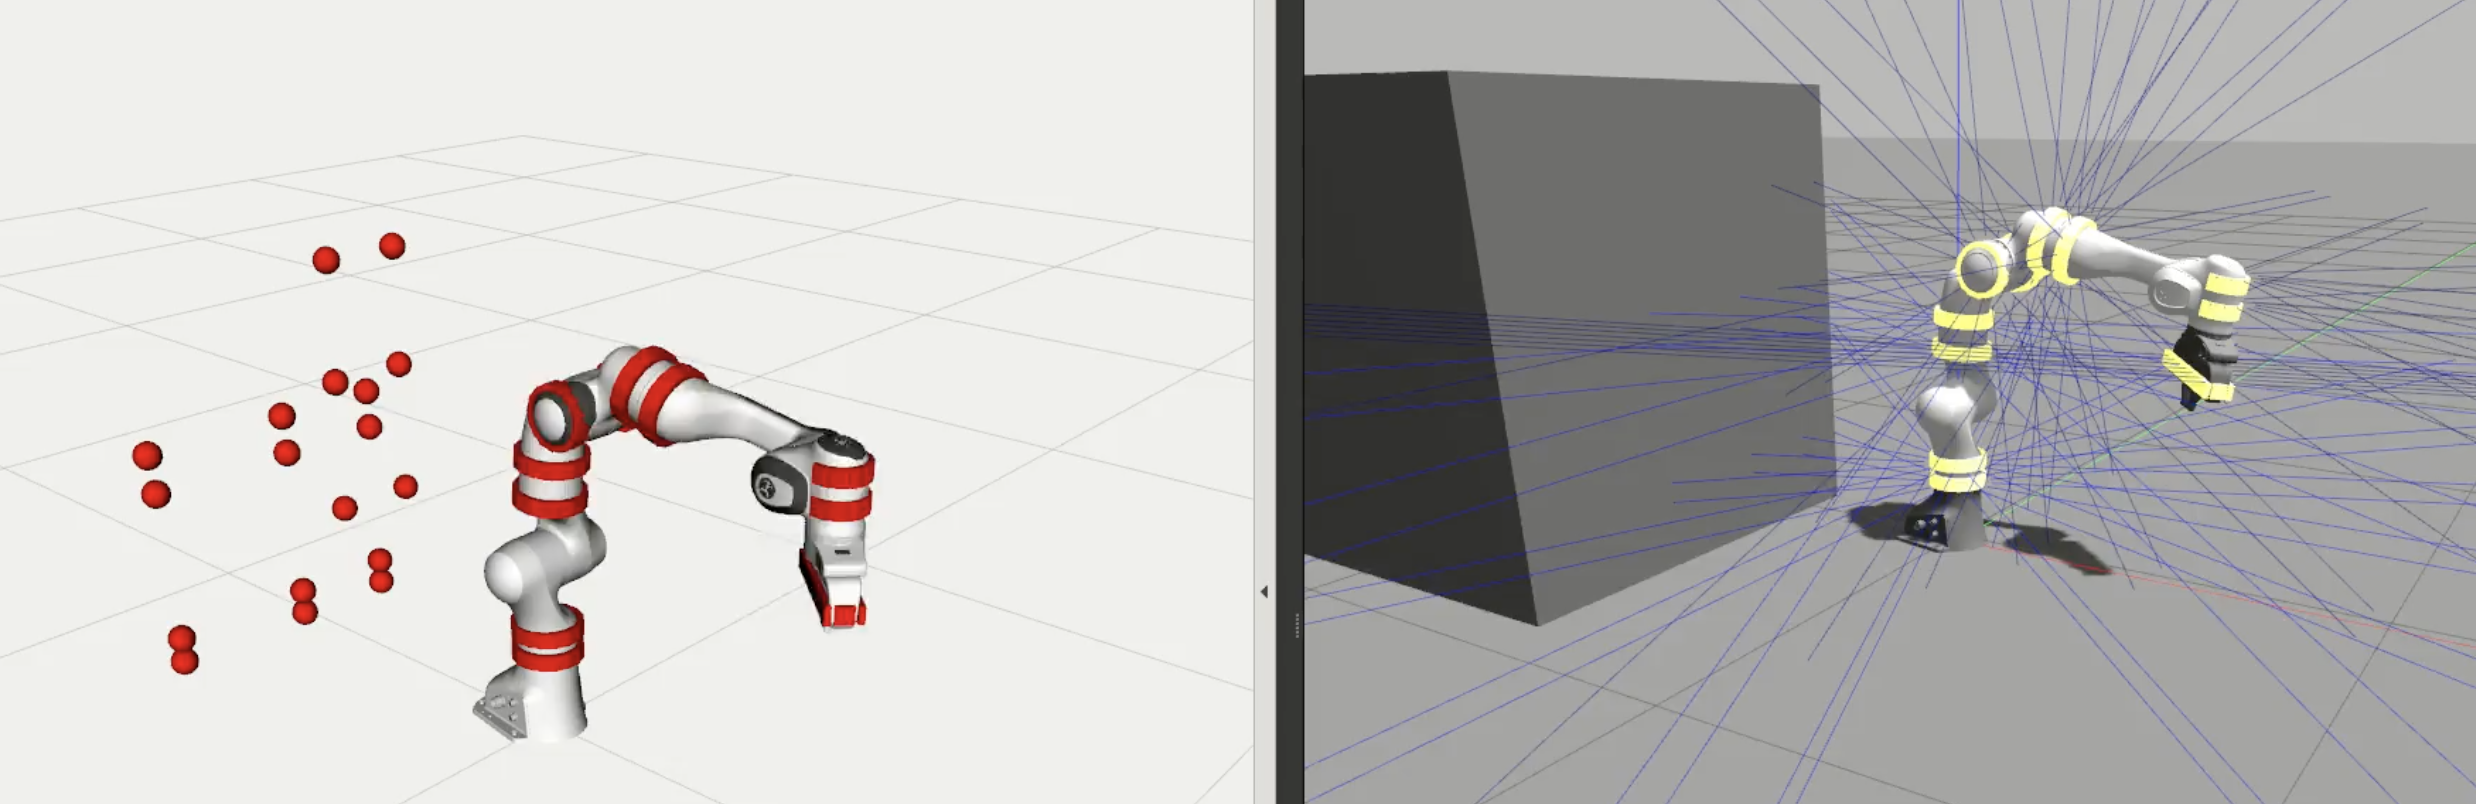
\includegraphics[width=\textwidth]{figs/visualizationpoints.png}
    \end{center}
\label{fig:visualizationpoints}
\end{figure}

\href{https://www.youtube.com/watch?v=nfT7xecq0Xo&list=PLnhdDYfKdsgimnQTQO-bmtKj-KRdbvGgS&index=2&t=0s}{This video} shows the same result in movement. Note that the perception is instantaneous. \lstinline{Gazebo} updates the position of the box when the left button of the mouse is released and this is the precise time that the old red spheres are deleted from perception and the new ones are created.

The update rate achieved in simulation has been 100 Hz. In practical applications the rate is limited by the specific sensor's capabilites, as opposed to the fact that the limiting factor is the computer's processing time for depth sensors, sensors that traditionally have been use for the obstacle avoidance control.

The buffer size in the demonstration is 10. At \SI{100}{\hertz}, this buffer size means it holds the data for \SI{100}{\milli \second}.



\section{End effector position control using the general solution of Instantaneous Forward Kinematics}
\label{s:resultsposition}

Cartesian position control, final code has been shown in section \ref{sss:eepositioncontrol}, was a necessary step to implement the rest of the avoidance algorithms. We have used many elements implemented in this controller as a foundation and to inform the movement of all subsequent controllers.

\href{https://www.youtube.com/watch?v=o4eRN95Fb8s&list=PLnhdDYfKdsgimnQTQO-bmtKj-KRdbvGgS&index=3&t=0s}{This video} presents the control in action. The desired trajectory is composed of 4 points that pertain to a circunference in the $x = \SI{0.5}{\metre}$ plane. This video presents the experiment that will be conducted for a first evaluation of the avoidance algorithm. The red point represents an obstacle and obviously it is not avoided in the case of this simple controller.

The gradient of the objective function that represents how close the joints are with respect to their mid range value, that goes into the second term of equation \ref{eq:generalsolution}, is a key element in this controller. If this them was omitted, weird joint configurations can be reached. As shown in figure \ref{fig:pandafloor} and \href{https://www.youtube.com/watch?v=JcoRfB1JB88&list=PLnhdDYfKdsgimnQTQO-bmtKj-KRdbvGgS&index=4&t=0s}{This video}, starting from a good initial position everything seems to work well in the beginning. However, at the second half of the video the arm reaches an undesired configuration in which it is near to hit the ground. This happens because of all posible joint velocities the minimum is being selected and this does not always involve the best solution. For a more detailed explanation on how the gradient works see section \ref{sss:IIK}.

\begin{figure}[H]
    \caption[pandafloor]{
    Panda with the gradient method deactivated.
    }
    \begin{center}
    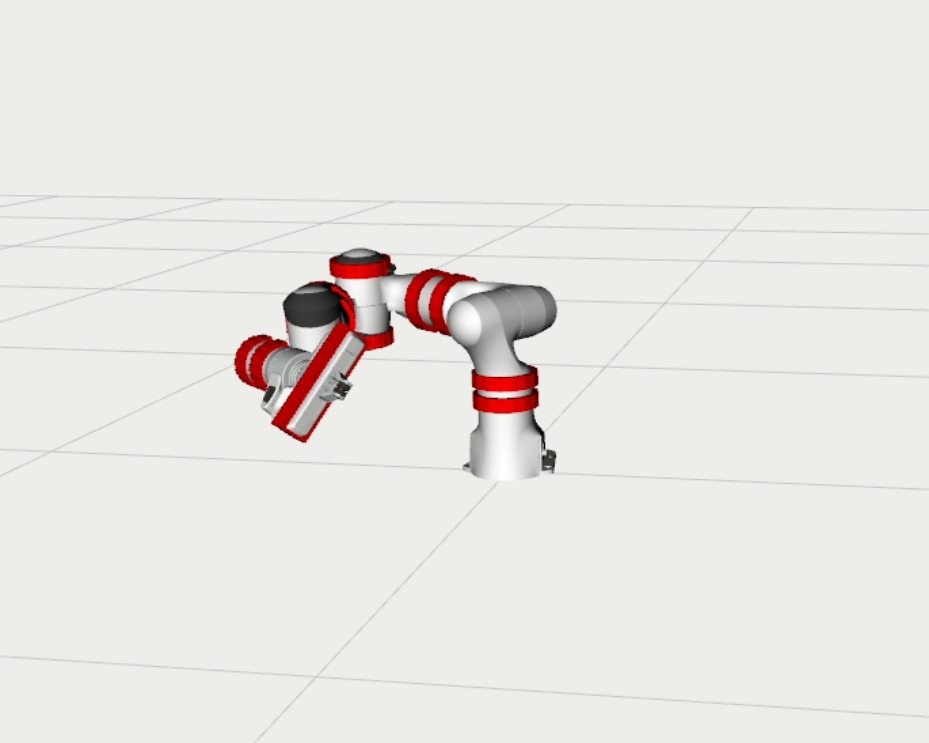
\includegraphics[width=110mm]{figs/pandafloor.png}
    \end{center}
\label{fig:pandafloor}
\end{figure}

Another important result is that, in listing \ref{code:noAvoidance}, if the threshold that decides if the main position control loop is complete is too small, the sensor update interval is not fast enough to ensure that level of precision. The velocity commanded to the end effector also needs to be considered, since for higher velocities a greater amount of distance is covered in the same amount of time. For example, when this threshold is set to less than $\SI{1}{\centi \metre}$ for an end effector speed of $\SI{0.35}{\metre/\second}$ , the final part of the trajectory sometimes becomes sloppy.

This threshold method is not the best one to solve the problem of trajectory control. A more advanced control method has been developed for the future development of the project. In contrast, it is a valid method for an initial checking of the behavior of the avoidance algorithms.

\section{Collision avoidance algorithm based on potential field methods and joint velocity constraints}

The approach explained in section \ref{ss:flacco} divided the avoidance control into two parts. One for the end effector and another one for the rest of the robot's body. We will demonstrate how this approach works in two parts. Firstly, the end effector algorithm will be tested independently. Then, the experiment presented in section \ref{s:resultsposition}

In \href{https://www.youtube.com/watch?v=wuBuytagogg&list=PLnhdDYfKdsgimnQTQO-bmtKj-KRdbvGgS&index=5&t=0s}{this video} we show an example of the repulsive vector modifying the trajectory of the end effector. The experiment is simple: the end effector is commanded an iterative movement between two points in a line parallel to the $x$ axis. An obstacle is placed in the trajectory.

The result is that the repulsive vector modifies the trajectory in the beginning and successfully moves around the object. When moving torwards the second objective the end effector stops when the desired velocity and the repulsive vector are exactly the same but with opposite directions. This represents a local minimum of the problem, since the desired position is actually reachable while avoiding the obstacle.

In \href{https://www.youtube.com/watch?v=pIpwVOOHptI&list=PLnhdDYfKdsgimnQTQO-bmtKj-KRdbvGgS&index=6&t=0s}{this other video}, the repulsive method is combined with the joint restriction method and tested with the aforementioned experiment (following a trajectory between 4 points). The obstacle is now succesfully avoided. However, it can be observed how the joint restrictions sometimes limit movements that do not have to be limited.

Acceleration limits (section \ref{sss:kinematiclimits}) have also been proven to be an important part of the correct behavior of the control. In the process of implementation, fast changes in the repulsive vector's direction resulted in jerky movements. Limiting acceleration has been proven to be a suitable solution to this fact.

The methods demonstrated in the next sections will improve this limitation imposed by the restrictions that prevent collision.

\section{Alternative approach to collision avoidance based on linear inequalities}

The approach explained in section \ref{ss:optimization} is different in two main ways with respect to Flacco. Control points where dynamically calculated for every obstacle point. The original desired end effector velocity was maintained as long as possible, as opposed to using repulsive vectors.

\href{https://www.youtube.com/watch?v=eJjqcIr-7Qw&list=PLnhdDYfKdsgimnQTQO-bmtKj-KRdbvGgS&index=7&t=0s}{In this video} the behaviour of the controller is shown. The first time the robot arm approaches the obstacle the avoidance is satisfactory. The second time something different happens. The movement torwards the next trajectory point is not allowed by the restrictions. The reason why this takes place is obvious if we analyze the second restriction (section \ref{sss:secondrestriction}). As we explained there, an overall increase in the distance to the obstacles is pursued by that restriction. In this case, as there is one single obstacle, it is the distance to that obstacle that is forced to increase. That is why the robot arm is not allowed to advance in the trajectory, there is no way to do so while satisfying the restriction.

On the other hand, another anomaly can be observed in the movement of the robot. After avoiding the obstacle for the first time, the position of the arm stays in the position adopted in order to avoid the obstacle. This effect was also observable in the previous control approach. What makes the robot approach the ground in figure \ref{fig:pandafloor} is the reason why this happens. The general solution shown in equation \ref{eq:generalsolution} and the gradient that minimizes the distance from the joint angles to their mid ranges are not being used in this section. In fact, the optimization selects the minimum norm joint velocity. This is exactly what happened if the second term of the general solution was deleted.

In addition, acceleration limitation is also very important in this section. The behaviour thanks to these limitations is more predictable and safer.

\section{Improvements to the collision avoidance control}
\label{s:improvements}

The restriction that causes the undesired behaviour in the previous test can be deleted. We have shown its implications are not convenient. Furthermore, we think that the restriction of the approach velocity is enough for if exploited properly. In section \ref{sss:firstrestriction}, we explained why the form of these restrictions are a suitable way of describing the avoidance problem. They allow setting up a repulsive action for any point in the robot when needed. This implies that the implications of the repulsive vectors applied to the end effector in section \ref{ss:flacco} can be extended to the rest of the body.

The original problem of maintaining the task as long as it is possible is also better described by this formulation, since the commanded velocity will be the original task velocity. That is, no repulsive vectors will modify the original task velocity. Since this goes in the optimization function, when it is not possible to maintain the original velocity, the closest possible velocity will be commanded.

In conclusion, the control proposed in this work is similar to the one presented in section \ref{ss:optimization}, but it is a more fundamental formulation of the original description of the problem.

The graph used to model the repulsive actions in the original publication (figure \ref{fig:plotxai}) has been enhanced for a more natural behaviour (figure \ref{fig:enhancedxai}). See \href{https://www.desmos.com/calculator/q2qofyanu9}{this interactive graph} for a deeper understanding of the parameters. Instead of using a linear graph we propose using exponential functions. In addition we propose that there are two thresholds for making decisions: the distance at which the control starts taking into account the obstacle: $d_{noticeable}$ and the distance at which repulsive actions start to be considered $d_{critical}$.

\begin{figure}[H]
    \caption[pandafloor]{
        Enhanced determination of $\dot{x}_{\mathrm{a}, i}$ as a function of $\|\mathbf{d_i}\|$.
    }
    \begin{center}
    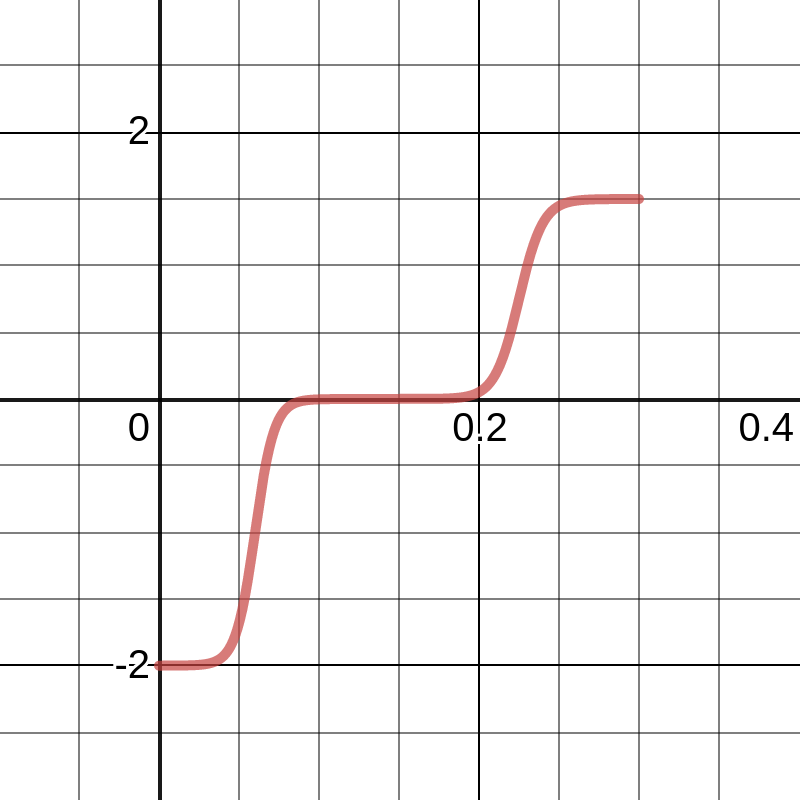
\includegraphics[width=110mm]{figs/desmos-graph.png}
    \end{center}
\label{fig:enhancedxai}
\end{figure}

The result of this enhanced approach can be observed \href{https://www.youtube.com/watch?v=iOytgdoOnlA&list=PLnhdDYfKdsgimnQTQO-bmtKj-KRdbvGgS&index=8&t=0s}{in this video}.

\section{Collision avoidance control in the real robot}

All the implementations and experiments described in the document so far have been done in simulation. The final will be to verify all the control algorithms work as well in the real Franka Panda Emika.

\href{https://www.youtube.com/watch?v=w5qdT06HPiU&list=PLnhdDYfKdsgimnQTQO-bmtKj-KRdbvGgS&index=8}{This video} shows the same experiment carried on in the last section, but in real life.

The perception algorithm explained in \ref{s:perception} has not been tested. The development of the artificial skin has been parallel to this work and as of the day of completion, the electronics of the sensors are in their third version and waiting to be tested. The kinematic calibration method, in contrast, has been succesfully tested using individual \textit{IMU} sensors.

The obstacle in the video has been placed manually via de command line tool \lstinline{rostopic pub}. We show the location of the point with our hand.